\documentclass[10pt,a4paper]{article}
\usepackage{needspace}
\usepackage[nobottomtitles]{titlesec}
\usepackage{multicol}
\usepackage{xcolor}
\usepackage{fp}
\usepackage{xfp}
\usepackage{enumitem}
\usepackage[version=4]{mhchem}
\usepackage{WriteOnGrid}
\usepackage{frcursive}
\usepackage{csvsimple}%
\usepackage[francais,bloc]{automultiplechoice}

\FPseed=10

\baremeDefautS{e=0,v=0,b=1,m=-.1}
\baremeDefautM{e=0,v=0,b=.5,m=-.1}

\graphicspath{ {./images/} }

\newenvironment{reponsesd}{
    \begin{multicols}{2}
    \begin{reponses} }{
    \end{reponses}
    \end{multicols}
}

\setlength{\columnseprule}{1pt}
\def\columnseprulecolor{\color{lightgray}}%

\let\oexplain\explain
\renewcommand{\explain}[1]{\oexplain{\textcolor{red}{#1}}}

\titleformat{\section}
  {\centering\hrule\vspace{2mm}}
  {\thesection}
  {1em}
  {}
  [\vspace{1mm}\hrule]

\titleformat{\subsection}
  {\em}
  {\thesubsection}
  {1em}
  {}

\newcommand{\sujet}{
\exemplaire{1}{%

\AMCsetFoot{\niveau{} \classe{} -- \prenom{}~\nom{} -- \thepage}

%%% debut de l'en-tête des copies :
\begin{center}
\vfill
\noindent{\large \bf Classe de \niveau{}°\classe{}}

\vspace*{3mm}

{\Large\bf Évaluation de compétences (non notée) STL - Physique-Chime 15/10/2025}

\vfill
\namefield{\noindent{}\fbox{\vspace*{3mm}
         \Huge\bf\prenom{}~\nom{}\normalsize{}%
         \vspace*{3mm}
      }}
\end{center}
\vfill

\begin{center}
\textbf{Durée : 30 minutes.}
\vspace*{5mm}

  Aucun document n'est autorisé.
  L'usage de la calculatrice est interdit.

  Les questions faisant apparaitre le symbole \multiSymbole{} peuvent
  présenter une ou plusieurs bonnes réponses. Les autres ont
  une unique bonne réponse.

  {\color{white} Des points négatifs seront affectés aux mauvaises réponses.}
  \vspace*{5mm}

  \textbf{IMPORTANT: Utilisez un crayon de papier bien noir pour cocher les cases, et une gomme pour effacer délicatement en cas d'erreur. Ne raturez pas les cases. Si vous effacez le pourtour de la case, ne le redessinez pas!}

  \vspace*{5mm}

  Ne pas faire comme ceci (pas centré, trop pâle, raturé):\\
  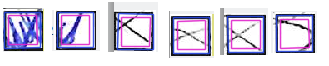
\includegraphics[width=4cm]{checkbox_bad.png}

  Mais comme cela (bien centré, bien foncé):\\
  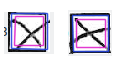
\includegraphics[width=2cm]{checkbox_good.png}

  Si vous faites une erreur et que vous ne pouvez effacer, raturez la case bien ostensiblement.

\end{center}
\vspace{1ex}
\vfill
\pagebreak
%%% fin de l'en-tête

\restituegroupe{groupes}


\AMCassociation{\id}

	  } % End \exemplaire{1}{%
} % End \newcommand{\sujet}{


%%%%§§§§§§§§§§§§§§§§§§§§§§§§§§§§§§§§§
\newcommand{\allq}{}
\newcommand{\nball}[1]{#1}

\begin{document}
%%%Options
\AMCrandomseed{10}

\def\AMCformQuestion#1{{\sc Question #1 :}}

\setdefaultgroupmode{withoutreplacement}
%%% Fin Options

%%% elements

\element{meta}{
  \begin{question}{meta1}\QuestionIndicative
    Pensez-vous poursuivre vos études dans un domaine lié à la physique, la chimie ou la biologie~?
    \begin{reponses}[o]
      \bonne{Oui}
      \bonne{Peut-être}
      \bonne{Ne sait pas}
      \bonne{Probablement pas}
      \bonne{Non}
    \end{reponses}
    \explain{C'est votre choix.}
  \end{question}

  \begin{question}{meta2}\QuestionIndicative
    Si oui, plutôt dans quel domaine (et sinon, quoi)~?
    \begin{reponses}[o]
      \bonne{Physique}
      \bonne{Chimie}
      \bonne{Biologie}
      \bonne{Autre, précisez: }
    \end{reponses}
    \explain{C'est votre choix.}
  \end{question}

  \begin{question}{meta3}\QuestionIndicative
    Que vous souhaitiez en faire votre métier ou non, aimez-vous la physique, la chimie ou la biologie~?
    \begin{reponses}[o]
      \bonne{Oui}
      \bonne{Un peu}
      \bonne{Ne sait pas}
      \bonne{Pas trop}
      \bonne{Non}
    \end{reponses}
    \explain{C'est votre choix.}
  \end{question}

  \begin{questionmult}{meta4}\QuestionIndicative
    Que préférez-vous (plusieurs choix possibles)~?
    \begin{reponses}[o]
      \bonne{Physique}
      \bonne{Chimie}
      \bonne{Biologie}
      \bonne{Mathématiques}
      \bonne{Autre, précisez: }
    \end{reponses}
    \explain{C'est votre choix.}
  \end{questionmult}

} % End \element{meta}{

\element{strspc}{
  \begin{questionmult}{strspc1}
    Une molécule est dite chirale si~:
    \begin{reponses}
      \mauvaise{ses atomes sont alignés}
      \mauvaise{elle est superposable à son image dans un miroir}
      \mauvaise{ses énantiomères sont diastéréoisométriques}
      \bonne{elle n'est pas superposable à son image dans un miroir}
    \end{reponses}
    \explain{un composé est dit chiral s'il n'est pas superposable à son 
    image dans un miroir plan.}
  \end{questionmult}
}

\element{strspc}{
  \begin{questionmult}{strspc2}
    La conformation d'une molécule se défini par~:
    \begin{reponses}
      \mauvaise{ses caractéristiques isomérique}
      \mauvaise{son respect des spécifications de son espèce chimique}
      \mauvaise{la qualité de son image dans un miroir plan}
      \bonne{les arangement des atomes tournant autour de liaisons simples}
    \end{reponses}
    \explain{La conformation d'une molécule correspond à l'orientation des atomes autour
    de liaisons simples. Celle-ci pouvant la plupart du temps tourner librement, 
    le même composé chimique peut passer de une à l'autre facilement.}
  \end{questionmult}
  }

\element{strspc}{
  \begin{questionmult}{strspc3}
    La configuration d'une molécule est~:
    \begin{reponses}
      \mauvaise{la version de système d'exploitation installé par défaut}
      \mauvaise{les arangement des atomes tournant autour de liaisons simples}
      \mauvaise{son image dans un miroir plan}
      \bonne{la disposition de ses atomes dans l'espace indépendamment des rotations
      autour des liaisons simples}
    \end{reponses}
    \explain{La configuration d'une molécule correspond à l'orientation des atomes dans l'espace,
    indépendamment des rotations autour des liaisons simples. Pour changer de configuration,
    il faut casser des liaisons pour en reformer d'autres.}
  \end{questionmult}
}

\element{strspc}{
  \begin {questionmult}{strspc4}
    Deux molécules sont des stéréo-isomères chimiques, si~:
    \begin{reponses}
      \mauvaise{elles ont une formule brute différente mais les mêmes propriétés chimiques}
      \mauvaise{elles ont la même conformation}
      \mauvaise{elles ont la meme configuration mais une formule semi-développée differente}
      \bonne{elles ont même formule semi-développée mais une configuration différente}
    \end{reponses}
    \explain{Les stéroisomères chimiques sont des molécules ayant la même formule
    semi-développée mais une conformation ou une configuration différente.}
  \end {questionmult}
}

\element{strspc}{
  \begin {questionmult}{strspc5}
    Deux molécules sont des énantiomères chimiques, si~:
    \begin{reponses}
      \mauvaise{elles ont même formule semi-développée mais ne sont pas images de l'une de l'autre dans un miroir plan}
      \mauvaise{elles ont la même mère}
      \mauvaise{la rotation de leur image dans un miroir dessine une ligne de symétrie}
      \bonne{elles sont images de l'une de l'autre dans un miroir plan}
    \end{reponses}
    \explain{Les enantiomères chimiques sont des molécules qui sont images de l'une de
    l'autre dans un miroir plan.}
  \end {questionmult}
}

\element{strspc}{
  \begin {questionmult}{strspc6}
    Deux molécules sont des diastéréoisométriques chimiques, si~:
    \begin{reponses}
      \mauvaise{elles ont une formule brute differente mais sont images de l'une de l'autre dans un miroir plan}
      \mauvaise{elles sont très très malades}
      \mauvaise{elles sont images de l'une de l'autre dans un miroir plan}
      \bonne{elles ont même formule semi-développée mais ne sont pas images de l'une de l'autre dans un miroir plan}
    \end{reponses}
    \explain{Les diastéréoisométriques .}
  \end {questionmult}
}

\element{nec}{
  \begin{questionmult}{nec1}
    À quoi servent les règles de Cahn, Ingold et Prelog en nomenclature chimique ?
    \begin{reponses}
      \mauvaise{Déterminer la conformation d'une molécule}
      \mauvaise{Établir les propriétés physiques d'un composé}
      \mauvaise{Déterminer si une molécule est chirale}
      \bonne{Donner la priorité aux substituents pour nommer les composés}
    \end{reponses}
    \explain{Les règles de Cahn-Ingold-Prelog permettent d'attribuer un ordre de priorité aux substituents afin de nommer correctement les composés chimiques.}
  \end{questionmult}
}

\element{nec}{
  \begin{questionmult}{nec2}
    Selon les règles de Cahn-Ingold-Prelog, comment détermine-t-on la priorité des substituents ?
    \begin{reponses}
      \mauvaise{En fonction du nombre de lettres dans le nom du substituant}
      \mauvaise{En fonction de la taille du substituant}
      \mauvaise{En fonction de la charge électrique du substituant}
      \bonne{En fonction du numéro atomique du premier atome du substituant}
    \end{reponses}
    \explain{La priorité est déterminée par le numéro atomique du premier atome du substituant. Si nécessaire, on examine les atomes suivants dans le substituant.}
  \end{questionmult}
}

\element{nec}{
  \begin{questionmult}{nec3}
    Qu'est-ce que la configuration R/S d'un centre chiral ?
    \begin{reponses}
      \mauvaise{Une classification des molécules en fonction de leur poids moléculaire}
      \mauvaise{Un système de désignation des isomères Z/E}
      \mauvaise{Une échelle de mesure de la polarité d'une molécule}
      \bonne{Un moyen de décrire l'arrangement spatial des substituents autour d'un atome}
    \end{reponses}
    \explain{La configuration R/S décrit l'arrangement tridimensionnel des quatre substituants différents autour d'un atome de carbone asymétrique.}
  \end{questionmult}
}

\element{nec}{
  \begin{questionmult}{nec4}
    Qu'est-ce que les désignations Z et E pour une double liaison ?
    \begin{reponses}
      \mauvaise{Elles indiquent si la molécule est droite ou gauche}
      \mauvaise{Elles classifient les molécules en fonction de leur solubilité}
      \mauvaise{Elles indiquent si la molécule est liquide ou gazeuse}
      \bonne{Elles décrivent la répartition des substituents de haute priorité autour d'une double liaison}
    \end{reponses}
    \explain{Z (zusammen) signifie que les substituents de plus haute priorité sont du même côté, tandis que E (entgegen) signifie qu'ils sont des côtés opposés.}
  \end{questionmult}
}

\element{acide}{
  \begin{questionmult}{acide1}
    Qu'est-ce qu'une constante d'équilibre acido-basique ?
    \begin{reponses}
      \mauvaise{Un paramètre qui mesure la vitesse d'un réaction chimique.}
      \mauvaise{Une valeur qui indique la température à laquelle une substance se décompose.}
      \mauvaise{C'est une unité de mesure pour les échelles de pH.}
      \bonne{Une constante qui décrit l'équilibre entre une espèce acide et 
      sa base conjuguée en solution aqueuse.}
    \end{reponses}
    \explain{La constante d'équilibre acido-basique est utilisée pour 
    quantifier la force relative d'un acide ou d'une base.}
  \end{questionmult}
}

\element{acide}{
  \begin{questionmult}{acide2}
    Qu'est-ce que le pKa, et à quoi sert-il ?
    \begin{reponses}
      \mauvaise{C'est un indicateur de la basicité d'une substance.}
      \mauvaise{C'est une mesure de la solubilité d'un composé dans l'eau.}
      \mauvaise{C'est l'abréviation pour 'pourquoi Kévin aime les acides'.}
      \bonne{C'est le logarithme négatif de la constante de dissociation acide, 
      servant à indiquer la force de l'acide.}
    \end{reponses}
    \explain{Un pKa élevé correspond à un faible acide, tandis qu'un pKa bas 
    indique un acide fort.}
  \end{questionmult}
}

\element{acide}{
  \begin{questionmult}{acide3}
    Comment le coefficient de dissociation est-il lié à la force d'un acide ?
    \begin{reponses}
      \mauvaise{Il n'y a pas de relation directe entre les deux.}
      \mauvaise{Un grand coefficient de dissociation indique un acide faible.}
      \mauvaise{Il est utilisé pour mesurer la quantité d'électricité dans une solution.}
      \bonne{Un grand coefficient de dissociation signifie que l'acide
      se dissocie plus facilement, ce qui en fait un acide fort.}
    \end{reponses}
    \explain{Le coefficient de dissociation reflète la proportion dans
    laquelle l'acide se sépare en ions en solution. Plus il est élevé, plus l'acide est fort.}
  \end{questionmult}
}

\element{acide}{
  \begin{questionmult}{acide4}
    Si un acide a un pKa de 5, qu'en déduisons-nous ?
    \begin{reponses}
      \mauvaise{Il s'agit d'un acide fort.}
      \mauvaise{Il est incapable de réagir avec une base.}
      \mauvaise{C'est un acide qui ne réagit qu'avec des bases naturelles.}
      \bonne{C'est un acide modérément faible}
    \end{reponses}
    \explain{Un pKa moyen comme 5 indique que l'acide n'est que très partiellement dissocié,
    ce qui est typique des acides faibles.}
  \end{questionmult}
}

\element{acide}{
  \begin{questionmult}{acide5}
    Quelle relation existe-t-il entre le pKa et la force d'un acide ?
    \begin{reponses}
      \mauvaise{Plus le pKa est élevé, plus l'acide est fort.}
      \mauvaise{Il n'y a pas de relation directe.}
      \mauvaise{Plus le pKa est élevé, plus l'acide est faible.}
      \bonne{Plus le pKa est bas, plus l'acide est fort.}
    \end{reponses}
    \explain{Un pKa bas signifie que l'acide se dissocie plus 
    facilement, ce qui en fait un acide fort.}
  \end{questionmult}
}

\element{acide}{
  \begin{questionmult}{acide6}
    Pourquoi les acides faibles ont-ils un coefficient de dissociation inférieur à 1 ?
    \begin{reponses}
      \mauvaise{Parce qu'ils ne sont pas capables de se dissocier.}
      \mauvaise{Parce que leur pKa est trop élevé.}
      \mauvaise{Parce qu'ils sont timides et n'osent pas se dissocier complètement.}
      \bonne{Parce qu'ils ne se dissocient pas complètement en solution aqueuse}
    \end{reponses}
    \explain{Les acides faibles partiellement se dissociie, donc leur coefficient
     de dissociation reste inférieur à 1.}
  \end{questionmult}
}


\element{tpco}{
  \begin{questionmult}{tpco1}
    Quelle est la principale fonction d'une solution tampon ?
    \begin{reponses}
      \mauvaise{Neutraliser complètement les acides et les bases forts.}
      \mauvaise{Agir comme catalyseur dans les réactions chimiques.}
      \mauvaise{Augmenter la conductivité électrique de l'eau.}
      \bonne{Résister aux changements de pH lorsqu'on ajoute de petites quantités
      d'acide ou de base.}
    \end{reponses}
    \explain{Les solutions tampon résistent aux variations du pH 
    en neutralisant les ions ajoutés grâce à leurs composants acido-basiques.}
  \end{questionmult}
}

\element{tpco}{
  \begin{questionmult}{tpco2}
    Comment les solutions tampon sont-elles généralement préparées ?
    \begin{reponses}
      \mauvaise{En mélangeant un acide fort avec une base forte.}
      \mauvaise{En ayant un certificat dûment tamponné.}
      \mauvaise{En dissolvant un solide dans l'eau pour créer une solution saturée.}
      \mauvaise{En chauffant un mélange d'acide et de base jusqu'à ébullition.}
      \bonne{En mélangeant un acide faible avec sa base conjuguée ou une base 
      faible avec son acide conjugué.}
    \end{reponses}
    \explain{Les solutions tampon sont préparées en combinant un 
    acide faible et sa base conjuguée.}
  \end{questionmult}
}

\element{tpco}{
  \begin{questionmult}{tpco3}
    Quel est le rôle du système de tampon bicarbonaté dans le sang ?
    \begin{reponses}
      \mauvaise{Réguler la température corporelle.}
      \mauvaise{Réguler la pression du sang.}
      \mauvaise{Transporter l'oxygène dans tout le corps.}
      \mauvaise{Digérer les aliments dans le sang.}
      \bonne{Maintenir le pH sanguin en neutralisant les ions 
      hydrogène en excès grâce à l'ion bicarbonate.}
    \end{reponses}
    \explain{Le système bicarbonaté aide à maintenir un pH stable
    dans le sang en neutralisant les excès d'acide ou de base.}
  \end{questionmult}
}

\element{tpco}{
  \begin{questionmult}{tpco4}
    Que se passe-t-il lorsque le CO2 se dissout dans l'eau ?
    \begin{reponses}
      \mauvaise{Il forme un acide fort qui se dissocie complètement.}
      \mauvaise{Il ne réagit pas et reste sous forme de molécules de \ce{CO2}.}
      \mauvaise{Il ne retrouve plus sa maison.}
      \mauvaise{Il réagit avec l'eau pour produire de l'oxygène.}
      \bonne{Il se dissout partiellement pour former de l'acide carbonique,
       qui se dissocie ensuite en ions \ce{H+} et bicarbonate (\ce{HCO3-}).}
    \end{reponses}
    \explain{Le \ce{CO2} se dissous réagit avec l'eau pour former une petite 
    quantité d'acide carbonique, lequel se dissocie en ions \ce{H+} et \ce{HCO3-}.}
  \end{questionmult}
}

\element{tpco}{
  \begin{questionmult}{tpco5}
    Comment les solutions tampon maintiennent-elles la stabilité du 
    pH lorsque des acides ou des bases sont ajoutés ?
    \begin{reponses}
      \mauvaise{Elles neutralisent complètement l'acide ou la base ajouté.}
      \mauvaise{Elles jettent les acides et les bases par-dessus bord.}
      \mauvaise{Elles augmentent leur concentration pour dominer la substance ajoutée.}
      \mauvaise{Elles changent de couleur pour indiquer les variations du pH.}
      \bonne{Elles réagissent avec l'acide ou 
      la base ajouté pour consommer les ions \ce{H+} ou \ce{OH-} en excès.}
    \end{reponses}
    \explain{Les solutions tampon neutralisent les ajouts d'acide 
    ou de base en réagissant avec les ions \ce{H+} ou \ce{OH-} en excédentaires.}
  \end{questionmult}
}

\element{tpco}{
  \begin{questionmult}{tpco6}
    Pourquoi le système de tampon bicarbonaté est-il important dans les systèmes biologiques ?
    \begin{reponses}
      \mauvaise{Il est essentiel pour la photosynthèse chez les plantes.}
      \mauvaise{Il amortit les chocs lors d'une chutte.}
      \mauvaise{Il facilite la digestion des aliments dans l'estomac.}
      \mauvaise{Il est impliqué dans la transmission des signaux nerveux.}
      \bonne{Il aide à maintenir un pH stable dans le sang et 
      d'autres fluides corporels.}
    \end{reponses}
    \explain{Le système bicarbonaté est essentiel pour maintenir 
    l'équilibre acido-basique nécessaire aux processus biologiques vitaux.}
  \end{questionmult}
}


\element{redox}{
  \begin{question}{redox1}
    Qu'est-ce qu'un agent oxydant ?
    \begin{reponses}
      \mauvaise{Une substance qui se décompose pour libérer des électrons.}
      \mauvaise{Un individu qui défend la civilisation occidentale.}
      \mauvaise{Une substance qui fournit de l'oxygène à une réaction.}
      \bonne{ Une substance qui accepte des électrons et provoque l'oxydation d'une autre substance.}
    \end{reponses}
    \explain{Un agent oxydant est une substance qui accepte des électrons, entraînant ainsi l'oxydation d'une autre substance.}
  \end{question}
}

\element{redox}{
  \begin{question}{redox2}
    Comment équilibrer une réaction d'oxydoréduction en solution acide ?
    \begin{reponses}
      \mauvaise{En ajoutant des ions \ce{OH-} des deux côtés de l'équation.}
      \mauvaise{En n'équilibrant pas du tout, car cela est inutile.}
      \mauvaise{En utilisant uniquement \ce{H2O} pour équilibrer l'oxygène.}
      \bonne{En divisant la réaction en demi-réactions, puis en équilibrant les éléments, les ions \ce{H+} et \ce{H2O} au besoin.}
    \end{reponses}
    \explain{Équilibrer une réaction d'oxydoréduction en solution acide implique de diviser la réaction en demi-réactions, puis d'équilibrer les éléments, les ions H⁺ et H₂O au besoin.}
  \end{question}
}

\element{redox}{
  \begin{question}{redox3}
    Qu'est-ce que l'anode dans une pile voltaïque ?
    \begin{reponses}
      \mauvaise{Le terminal positif où se produit la réduction.}
      \mauvaise{Un type de pont salin dans la pile.}
      \mauvaise{L'anneau qui sert à la maintenir en place'}
      \bonne{Le terminal négatif où se produit l'oxydation.}
    \end{reponses}
    \explain{L'anode est le terminal négatif d'une pile voltaïque où se produit l'oxydation.}
  \end{question}
}

\element{redox}{
  \begin{question}{redox4}
    Quelle est la fonction d'un pont salin dans une cellule électrochimique ?
    \begin{reponses}
      \mauvaise{Il permet aux visiteurs de passer la rivière.}
      \mauvaise{Il sépare complètement les solutions.}
      \mauvaise{Il augmente la tension de la cellule.}
      \bonne{Il empêche le mélange des solutions tout en permettant la migration des ions.}
    \end{reponses}
    \explain{Le pont salin empêche le mélange des solutions tout en permettant la migration des ions, maintenant ainsi l'équilibre électrique.}
  \end{question}
}

\element{redox}{
  \begin{question}{redox6}
    Qu'est-ce qu'une demi-réaction ?
    \begin{reponses}
      \mauvaise{Une réaction montrant toutes les étapes.}
      \mauvaise{Une réaction sans transfert d'électrons.}
      \mauvaise{N'est applicable qu'en solutions basiques.}
      \bonne{Une représentation soit de la phase d'oxydation ou de réduction.}
    \end{reponses}
    \explain{Une demi-réaction est une représentation de l'oxydation ou de la réduction, impliquant des électrons.}
  \end{question}
}



\element{cichi}{
  \begin{question}{cichi2}
    Qu'est-ce que la constante de vitesse ($k$) représente dans une équation chimique ?
    \begin{reponses}
      \mauvaise{C'est la concentration initiale du réactif.}
      \mauvaise{C'est le temps nécessaire pour que la réaction se termine.}
      \mauvaise{C'est la température à laquelle la réaction se produit.}
      \bonne{C'est un facteur de proportionnalité qui dépend de la température et de la nature des réactifs.}
    \end{reponses}
    \explain{La constante de vitesse ($k$) est un facteur dans la loi de vitesse qui reflète combien vite la réaction se déroule dans des conditions spécifiques, influencé par des facteurs tels que la température et les espèces chimiques impliquées.}
  \end{question}
}

\element{cichi}{
  \begin{question}{cichi4}
    Quelle est l'expression de la demi-vie ($t_{\frac{1}{2}}$) pour une réaction du premier ordre (avec $[A]_0$ concentration initiale) ?
    \begin{reponses}
      \mauvaise{$t_{\frac{1}{2}} = [A]_0 / k$}
      \mauvaise{$t_{\frac{1}{2}} = 1 / (k [A]_0)$}
      \mauvaise{$t_{\frac{1}{2}} = k \times [A]_0$}
      \bonne{$t_{1/2} = \frac{\ln(2)}{k}$, et il est indépendant de la concentration initiale.}
    \end{reponses}
    \explain{Pour les réactions du premier ordre, la demi-vie est donnée par $t_{1/2} = \frac{\ln(2)}{k}$ et ne dépend pas de la concentration initiale du réactif.}
  \end{question}
}

\element{radio}{
  \begin{question}{radio1}
    Qu'est-ce qu'une émission alpha ($\alpha$)~?
    \begin{reponses}
      \mauvaise{Une émission alpha consiste en l'éjection d'un photon gamma haute énergie.}
      \mauvaise{Une émission alpha est la libération d'un neutron excité.}
      \mauvaise{Une émission alpha se produit lors de la capture d'un électron par un proton.}
      \bonne{Une émission alpha est le dégagement d'un noyau d'hélium (2 protons et 2 neutrons).}
    \end{reponses}
    \explain{Une émission alpha implique l'éjection d'un noyau d'hélium. Les autres options décrivent d'autres types de radiation.}
  \end{question}
}

\element{radio}{
  \begin{question}{radio2}
    Quelles sont les principales différences entre une émission bêta moins ($\beta^-$) et une émission bêta plus ($\beta^+$) ?
    \begin{reponses}
      \mauvaise{Une émission $\beta^-$ libère un positron, tandis qu'une émission $\beta^+$ libère un neutron.}
      \mauvaise{Une émission $\beta^-$ se produit dans des noyaux riches en neutrons.}
      \mauvaise{Une émission $\beta^-$ est moins pénétrante qu'une émission $\beta^+$.}
      \bonne{ Une émission $\beta^-$ libère un électron, tandis qu'une émission $\beta^+$ libère un positron.}
    \end{reponses}
    \explain{L'émission $\beta^-$ libère un électron et $\beta^+$ libère un positron (son antiparticule).}
  \end{question}
}

\element{radio}{
  \begin{question}{radio3}
    Qu'est-ce qu'une émission gamma ($\gamma$), et dans quel contexte se produit-elle ?
    \begin{reponses}
      \mauvaise{ Une émission $\gamma$ est l'éjection d'un noyau d'hélium.}
      \mauvaise{ Une émission $\gamma$ se produit lors de la capture d'un électron par un proton.}
      \mauvaise{ Une émission $\gamma$ libère un neutron excité.}
      \bonne{Une émission $\gamma$ est l'émission d'un photon haute énergie suite à une transition nucléaire.}
    \end{reponses}
    \explain{L'émission $\gamma$ implique l'émission de photons haute énergie lors d'une transition nucléaire.}
  \end{question}
}

\element{radio}{
  \begin{question}{radio4}
    Quelle loi physique est conservée lors d'une désintégration radioactive ?
    \begin{reponses}
      \mauvaise{ La masse atomique totale.}
      \mauvaise{ Le spin des particules émises.}
      \mauvaise{ L'énergie cinétique des produits de désintégration.}
      \bonne{ Le nombre de nucléions et l'énergie totale sont conservés.}
    \end{reponses}
    \explain{Lors d'une désintégration radioactive, le nombre de nucléons et l'énergie totale sont conservés. }
  \end{question}
}

\element{radio}{
  \begin{question}{radio5}
    Comment évolue la population moyenne d’un ensemble de noyaux radioactifs au fil du temps ?
    \begin{reponses}
      \mauvaise{ Elle augmente exponentiellement.}
      \mauvaise{ Elle reste constante.}
      \mauvaise{ Elle suit une décroissance logarithmique.}
      \bonne{ Elle diminue suivant une loi exponentielle.}
    \end{reponses}
    \explain{La population de noyaux radioactifs diminue suivant une décroissance exponentielle.}
  \end{question}
}

\element{radio}{
  \begin{question}{radio6}
    Qu'est-ce que la constante de désintégration $\lambda$, et quelle unité a-t-elle ?
    \begin{reponses}
      \mauvaise{ C'est la vitesse de décroissance en noyaux par seconde.}
      \mauvaise{ C'est la probabilité de désintégration par seconde, en pourcentage.}
      \mauvaise{ C'est la masse critique d'un matériau.}
      \bonne{ C'est la probabilité de désintégration par seconde.}
    \end{reponses}
    \explain{$\lambda$ représente la probabilité de désintégration par unité de temps (unité : $\text{s}^{-1}$).}
  \end{question}
}

\element{radio}{
  \begin{question}{radio7}
    Qu'est-ce que le temps de demi-vie d'un isotope radioactif ?
    \begin{reponses}
      \mauvaise{ Le temps de demi-vie est la durée pendant laquelle l'isotope est dangereux.}
      \mauvaise{ Le temps de demi-vie est la période après laquelle l'isotope disparaît complètement.}
      \mauvaise{ Le temps de demi-vie est une mesure de radioactivité.}
      \bonne{ Le temps de demi-vie est la durée après laquelle 50\% des noyaux radioactifs ont subi une désintégration.}
    \end{reponses}
    \explain{La demi-vie est la durée après laquelle 50\% des noyaux radioactifs ont subi une désintégration.}
  \end{question}
}

\element{radio}{
  \begin{question}{radio8}
    Qu'est-ce que l'activité d'un échantillon radioactif ?
    \begin{reponses}
      \mauvaise{ La quantité de rayonnement $\gamma$ émis.}
      \mauvaise{ Le nombre total de désintégrations depuis la formation de l'échantillon.}
      \mauvaise{ La dose de radiation reçue par un être humain à proximité.}
      \bonne{ Le nombre de désintégrations par seconde dans l'échantillon.}
    \end{reponses}
    \explain{L'activité correspond au nombre de désintégrations par unité de temps.}
  \end{question}
}

\element{motion}{
  \begin{question}{motion1}
    Qu'est-ce que la force électrostatique~?
    \begin{reponses}
      \mauvaise{Une force qui pousse les objets vers le bas.}
      \mauvaise{Une force qui fait tourner les objets.}
      \mauvaise{Une force qui fait cuire les aliments.}
      \bonne{Une force qui attire ou repousse les objets chargés électriquement.}
    \end{reponses}
    \explain{La force électrostatique est une interaction entre particules chargées, décrite par la loi de Coulomb. Elle peut attirer ou repousser selon les charges.}
  \end{question}
}

\element{motion}{
  \begin{question}{motion2}
    Qu'est-ce que le champ électrostatique~?
    \begin{reponses}
      \mauvaise{Un endroit où les particules ne s'approchent jamais.}
      \mauvaise{Une région où les champs magnétiques dominent.}
      \mauvaise{Un lieu idéal pour piqueniquer avec des pizzas.}
      \bonne{ Une zone autour d'un objet chargé où la force électrostatique peut être détectée.}
    \end{reponses}
    \explain{Le champ électrostatique représente la distribution de forces autour d'un objet chargé, mesuré en newtons par coulomb.}
  \end{question}
}

\element{motion}{
  \begin{question}{motion3}
    Pourquoi est-il important de dresser un bilan des forces~?
    \begin{reponses}
      \mauvaise{Pour savoir combien de force il faut pour soulever une montagne.}
      \mauvaise{Pour mesurer la résistance de l'air dans les tunnels.}
      \mauvaise{Pour vérifier si les objets sont vraiment inanimés.}
      \bonne{Pour déterminer les forces qui agissent sur un objet et leur équilibre.}
    \end{reponses}
    \explain{Le bilan des forces permet de comprendre comment les interactions physiques affectent un objet, essentiel pour analyser ses mouvements ou son équilibre.}
  \end{question}
}

\element{motion}{
  \begin{question}{motion4}
    Quelle est la première loi de Newton~?
    \begin{reponses}
      \mauvaise{Un objet en mouvement arrête de se déplacer sans force extérieure.}
      \mauvaise{La gravité attire tout vers le centre de la Terre.}
      \mauvaise{Tout ce qui est lisse ne peut rouiller.}
      \bonne{Sans force extérieure, un objet au repos reste au repos, et un objet en mouvement uniforme continue.}
    \end{reponses}
    \explain{La première loi de Newton décrit l'inertie, montrant que les objets maintiennent leur état de mouvement ou de repos à moins qu'une force ne les modifie.}
  \end{question}
}

\element{motion}{
  \begin{question}{motion5}
    Comment la chute verticale avec frottement visqueux affecte-t-elle un objet~?
    \begin{reponses}
      \mauvaise{En augmentant sa vitesse jusqu'à ce qu'il explose.}
      \mauvaise{En le faisant disparaître dans l'air.}
      \mauvaise{En le ralentissant progressivement jusqu'à l'arrêt.}
      \bonne{En exerçant une force de frottement proportionnelle à sa vitesse.}
    \end{reponses}
    \explain{Le frottement visqueux oppose la motion, proportionnellement à la vitesse, ralentissant l'objet et l'empêchant d'accélérer indéfiniment.}
  \end{question}
}

\element{motion}{
  \begin{question}{motion6}
    Qu'est-ce que le régime permanent~?
    \begin{reponses}
      \mauvaise{Un état où tout est en mouvement sans arrêt.}
      \mauvaise{Une situation où les forces s'équilibrent.}
      \mauvaise{Un moment où l'univers entier est en paix.}
      \bonne{ Une situation où la vitesse de l'objet devient constante malgré des forces opposées.}
    \end{reponses}
    \explain{Au régime permanent, les forces en jeu s'équilibrent, conduisant à une vitesse constante sans accélération.}
  \end{question}
}

\element{motion}{
  \begin{question}{motion7}
    Qu'est-ce que la vitesse en régime permanent~?
    \begin{reponses}
      \mauvaise{La vitesse maximale qu'un objet peut atteindre.}
      \mauvaise{La vitesse minimum pour éviter de tomber.}
      \mauvaise{La vitesse idéale pour cuisiner des œufs.}
      \bonne{ La vitesse constante atteinte quand la force motrice équilibre la résistance.}
    \end{reponses}
    \explain{En régime permanent, l'objet se déplace à une vitesse constante où la somme des forces est nulle, équilibrant poussée et frottement.}
  \end{question}
}

\element{energ}{
  \begin{question}{energ1}
    Qu'est-ce qu'une chaîne énergétique ?
    \begin{reponses}
      \mauvaise{Un ensemble de moteurs qui se relayent pour éviter la fatigue.}
      \mauvaise{Des outils utilisés en cuisine pour découper les légumes.}
      \mauvaise{Une série de transformations où l'énergie se multiplie à chaque étape.}
      \bonne{ Une succession d'étapes où l'énergie est transférée et transformée dans un système.}
    \end{reponses}
    \explain{Une chaîne énergétique décrit les différents processus par lesquels l'énergie est transférée et transformée à travers un système, de sa source à ses utilisations finales.}
  \end{question}
}

\element{energ}{
  \begin{question}{energ2}
    Quelle est la loi fondamentale de la conservation de l’énergie ?
    \begin{reponses}
      \mauvaise{L'énergie se crée et se détruit constamment dans la nature.}
      \mauvaise{La vitesse de l'énergie augmente avec la distance.}
      \mauvaise{Toute énergie finit par disparaître complètement.}
      \bonne{ La quantité totale d'énergie dans un système isolé reste constante, bien qu'elle puisse changer de forme.}
    \end{reponses}
    \explain{La conservation de l'énergie indique que l'énergie ne peut être créée ni détruite, seulement transformée ou transférée d'une forme à une autre.}
  \end{question}
}

\element{energ}{
  \begin{question}{energ3}
    Qu'est-ce que le rendement énergétique ?
    \begin{reponses}
      \mauvaise{Le rapport entre l'énergie perdue et l'énergie utile.}
      \mauvaise{La vitesse à laquelle l'énergie est transférée dans un système.}
      \mauvaise{Un type de transformation énergétique sans perte.}
      \bonne{ Le rapport entre l'énergie utile produite et l'énergie totale consommée.}
    \end{reponses}
    \explain{Le rendement énergétique est la proportion d'énergie utilisée de manière efficace par rapport à l'énergie totale disponible, souvent exprimé en pourcentage : $\eta = \frac{E_{utile}}{E_{totale}}$.}
  \end{question}
}

\element{energ}{
  \begin{question}{energ4}
    Qu’est-ce que la dissipation énergétique ?
    \begin{reponses}
      \mauvaise{Le processus par lequel l'énergie est stockée dans un système.}
      \mauvaise{La transformation totale de l'énergie en travail utile.}
      \mauvaise{ Une technique pour augmenter l'efficacité énergétique.}
      \bonne{ La perte d'énergie sous forme de chaleur ou de mouvement aléatoire, généralement due à la résistance ou au frottement.}
    \end{reponses}
    \explain{La dissipation énergétique correspond aux pertes d'énergie qui ne peuvent être récupérées ni utilisées pour un travail utile, souvent sous forme de chaleur.}
  \end{question}
}

\element{energ}{
  \begin{question}{energ5}
    Qu'est-ce qu’un transfert thermique ?
    \begin{reponses}
      \mauvaise{Un processus où la chaleur est générée mais ne se déplace jamais.}
      \mauvaise{ Une méthode pour stocker l'énergie chimique dans les aliments.}
      \mauvaise{Un type de mouvement des particules quantiques.}
      \bonne{ Le passage de la chaleur d'un corps à un autre ou d'une partie à une autre du même corps.}
    \end{reponses}
    \explain{Le transfert thermique se produit lorsque de la chaleur est échangée entre deux systèmes ou parties d'un système à des températures différentes.}
  \end{question}
}

\element{energ}{
  \begin{question}{energ6}
    Quelles sont les principales formes de transfert thermique ?
    \begin{reponses}
      \mauvaise{La conduction, la convection et la conversion.}
      \mauvaise{La radiation, l'isolation et la réflexion.}
      \mauvaise{La conduction, la convection et la créativité.}
      \bonne{ La conduction, la convection et la radiation.}
    \end{reponses}
    \explain{Les trois principales formes de transfert thermique sont la conduction (d'un corps à un autre en contact direct), la convection (via un fluide) et la radiation (par ondes électromagnétiques).}
  \end{question}
}




\element{meca}{
  \begin{question}{meca1}
    Qu'est-ce que le travail élémentaire d'une force ?
    \begin{reponses}
      \mauvaise{Le travail effectué par une force pour déplacer un objet.}
      \mauvaise{L'énergie potentielle stockée dans un champ de force.}
      \mauvaise{La quantité de café nécessaire pour bouger un objet lourd.}
      \bonne{L'énergie transférée lorsqu'une force fait déplacer un objet sur une distance.}
    \end{reponses}
    \explain{Le travail élémentaire d'une force correspond à l'énergie transférée 
    lorsque la force agit sur un objet et le déplace. Cela se calcule comme 
    $W = F \cdot d \cdot \cos(\theta)$, où $F$ est la force, $d$ est la distance et $\theta$ l'angle entre la force 
et le déplacement.}
  \end{question}
}


\element{meca}{
  \begin{question}{meca2}
    Qu'est-ce que le travail du poids ?
    \begin{reponses}
      \mauvaise{Le travail effectué par une personne pour soulever des haltères.}
      \mauvaise{L'énergie cinétique d'un objet en mouvement.}
      \mauvaise{La force nécessaire pour voler comme un super-héros.}
      \bonne{L'énergie transférée par la gravité lorsque l'objet change de hauteur.}
    \end{reponses}
    \explain{Le travail du poids est le travail effectué par la force gravitationnelle, 
    $W = m \cdot g \cdot h$, où $m$ est la masse, $g$ l'accélération gravitationnelle et $h$ la hauteur.}
  \end{question}
}

\element{meca}{
  \begin{question}{meca3}
    Qu'est-ce que l'énergie potentielle de pesanteur ?
    \begin{reponses}
      \mauvaise{L'énergie utilisée pour courir sur une pente.}
      \mauvaise{L'énergie stockée dans un ressort comprimé.}
      \mauvaise{La quantité d'énergie nécessaire pour ne plus jamais boire de café.}
      \bonne{L'énergie associée à la présence d'un objet dans un champ gravitationnel.}
    \end{reponses}
    \explain{L'énergie potentielle de pesanteur est donnée par $E_p = m \cdot g \cdot h$, où $m$ est la masse, 
    $g$ l'accélération gravitationnelle et $h$ la hauteur. Elle représente l'énergie stockée due à la position de l'objet.}
  \end{question}
}

\element{meca}{
  \begin{question}{meca4}
    Qu'est-ce que l'énergie mécanique ?
    \begin{reponses}
      \mauvaise{L'énergie utilisée pour réfléchir à une question difficile.}
      \mauvaise{La somme de l'énergie cinétique et de l'énergie thermique.}
      \mauvaise{La quantité d'énergie nécessaire pour faire fonctionner une machine à remonter le temps.}
      \bonne{La somme de l'énergie cinétique et de l'énergie potentielle d'un système.}
    \end{reponses}
    \explain{L'énergie mécanique est la combinaison de l'énergie cinétique 
    ($E_c = \frac{1}{2}mv^2$) et de l'énergie potentielle ($E_p = mgh$), représentant le total de l'énergie dans un système.}
  \end{question}
}

\element{meca}{
  \begin{question}{meca5}
    Qu'est-ce que la conservation de l'énergie ?
    \begin{reponses}
      \mauvaise{L'idée que l'énergie peut être créée ou détruite.}
      \mauvaise{La capacité à stocker de l'énergie pour une utilisation future.}
      \mauvaise{Un concept qui permet de faire disparaître l'énergie lorsqu'elle n'est plus utile.}
      \bonne{Le principe selon lequel l'énergie ne peut être créée ni détruite, seulement transformée.}
    \end{reponses}
    \explain{La conservation de l'énergie signifie que la quantité totale d'énergie
    dans un système isolé reste constante, même si elle change de forme (par exemple,
    de l'énergie potentielle en énergie cinétique).}
  \end{question}
}

\element{meca}{
  \begin{question}{meca6}
    Comment la puissance et l'énergie sont-elles liées ?
    \begin{reponses}
      \mauvaise{La puissance est une forme d'énergie stockée.}
      \mauvaise{L'énergie est la puissance divisée par le temps.}
      \mauvaise{La puissance est la quantité d'énergie disponible pour faire du travail.}
      \bonne{La puissance exprime la vitesse à laquelle l'énergie est utilisée ou transférée.}
    \end{reponses}
    \explain{La puissance représente le taux d'utilisation ou de transfert d'énergie,
    tandis que l'énergie est la quantité totale d'énergie disponible.
    Par exemple, $P = \frac{E}{t}$ montre comment la puissance est liée à l'énergie et au temps.}
  \end{question}
}

\element{meca}{
  \begin{question}{meca7}
    Qu'est-ce que l'énergie mécanique disponible ?
    \begin{reponses}
      \mauvaise{L'énergie perdue sous forme de chaleur.}
      \mauvaise{L'énergie potentielle stockée dans un champ magnétique.}
      \mauvaise{La quantité d'énergie nécessaire pour faire fonctionner une machine à remonter le temps.}
      \bonne{L'énergie totale (cinétique et potentielle) qui peut être utilisée pour effectuer un travail.}
    \end{reponses}
    \explain{L'énergie mécanique disponible fait référence à l'énergie totale
    d'un système qui peut être utilisée pour accomplir un travail, y compris à la fois l'énergie cinétique et potentielle.}
  \end{question}
}

\element{meca}{
  \begin{question}{meca8}
    Pourquoi la conservation de l'énergie est-elle importante ?
    \begin{reponses}
      \mauvaise{Parce qu'elle permet de créer de l'énergie gratuitement.}
      \mauvaise{Parce qu'elle explique pourquoi nous devons manger pour avoir de l'énergie.}
      \mauvaise{Parce qu'elle prédit que l'univers finira par manquer d'énergie.}
      \bonne{Parce qu'elle décrit comment l'énergie se transforme mais ne disparaît pas, aidant à comprendre les systèmes physiques.}
    \end{reponses}
    \explain{La conservation de l'énergie est cruciale car elle explique que
    toute énergie reste présente sous une forme ou une autre dans un système isolé,
    permettant de prédire et d'étudier divers phénomènes naturels.}
  \end{question}
}


\element{echi}{
  \begin{question}{echi1}
    Qu’est-ce qu’un diagramme d’état d’un corps pur ?
    \begin{reponses}
      \mauvaise{Un graphique montrant l’évolution des prix d’un corps sur le marché.}
      \mauvaise{Un schéma représentant les différents états d’humeur d’une personne.}
      \mauvaise{Un tableau périodique des éléments chimiques.}
      \bonne{LUn graphique des différentes phases en fonction de la température et de la pression.}
    \end{reponses}
    \explain{Un diagramme d’état montre les conditions de température et de pression 
    auxquelles un corps pur se trouve sous différentes phases (solide, liquide ou gazeux). 
    Il est essentiel pour comprendre les transitions de phase.}
  \end{question}
}

\element{echi}{
  \begin{question}{echi2}
    Comment déterminez-vous le point triple sur un diagramme d’état ?
    \begin{reponses}
      \mauvaise{En suivant la ligne des températures négatives.}
      \mauvaise{En trouvant l’intersection des axes X et Y.}
      \mauvaise{En comptant les étoiles sur le graphique.}
      \bonne{À l’intersection des trois courbes de fusion, sublimation et condensation.}
    \end{reponses}
    \explain{Le point triple est le point spécifique sur un diagramme d’état où les pressions 
    et températures permettent aux trois phases (solide, liquide et gazeux) de coexister en équilibre.}
  \end{question}
}

\element{echi}{
  \begin{question}{echi3}
    Définissez l’enthalpie de changement d’état.
    \begin{reponses}
      \mauvaise{L’énergie libérée par une réaction chimique à pression constante.}
      \mauvaise{La quantité de chaleur perdue par un corps en mouvement.}
      \mauvaise{Un type de cuisson à basse température.}
      \bonne{L'énergie transférées lors d’un changement d'état (à T° constante).}
    \end{reponses}
    \explain{L’enthalpie de changement d’état représente la quantité de chaleur échangée 
    lorsqu’une substance change de phase à température constante, comme la fusion de la glace en eau.}
  \end{question}
}

\element{echi}{
  \begin{question}{echi4}
    Comment calculez-vous la chaleur requise pour un changement d’état en utilisant une enthalpie de changement d'état (en J/kg)?
    \begin{reponses}
      \mauvaise{En multipliant cette enthalpie par le volume du corps.}
      \mauvaise{En divisant cette enthalpie par la température ambiante.}
      \mauvaise{En soustrayant cette enthalpie de celle de la température initiale.}
      \bonne{En multipliant la masse du corps par cette enthalpie.}
    \end{reponses}
    \explain{La chaleur requise pour un changement d’état est calculée en multipliant 
    la masse de la substance par l'enthalpie de changement d'état du processus.}
  \end{question}
}

\element{echi}{
  \begin{question}{echi5}
    Définissez l’enthalpie standard de formation.
    \begin{reponses}
      \mauvaise{L’énergie libérée par la combustion d’un combustible.}
      \mauvaise{La quantité de chaleur perdue lors du refroidissement d’une substance.}
      \mauvaise{Un type de réaction chimique exothermique.}
      \bonne{L’énergie échangée pour former un composé à partir de ses éléments constitutifs.}
    \end{reponses}
    \explain{L’enthalpie standard de formation est la variation d’enthalpie qui accompagne 
    la formation d’un mole d’un composé à partir de ses éléments constitutifs dans leurs états 
    standards, sous pression atmospérique.}
  \end{question}
}

\element{echi}{
  \begin{question}{echi6}
    Comment utilisez-vous la loi de Hess pour calculer l’enthalpie standard de réaction ?
    \begin{reponses}
      \mauvaise{En additionnant toutes les enthalpies de formation des réactifs.}
      \mauvaise{En soustrayant l’enthalpie des produits de celle des réactifs.}
      \mauvaise{En multipliant l’enthalpie par le nombre de moles.}
      \bonne{En soustrayant la somme des enthalpies de formation des 
      réactifs de celle des produits.}
    \end{reponses}
    \explain{La loi de Hess permet de calculer l’enthalpie standard d’une réaction en soustrayant 
    la somme des enthalpies standard de formation des réactifs de celle des produits.}
  \end{question}
}

\element{echi}{
  \begin{question}{echi7}
    Qu’est-ce que la capacité thermique~?
    \begin{reponses}
      \mauvaise{La capacité à résister aux hautes températures.}
      \mauvaise{La quantité de chaleur requise pour chauffer un corps sans changement de phase.}
      \mauvaise{Un type de thermostat pour réguler la température.}
      \bonne{La quantité de chaleur nécessaire pour élever la température d’un corps.}
    \end{reponses}
    \explain{La capacité thermique représente la chaleur requise pour modifier la température d’une unité de masse d'un corps. 
    Elle est exprimée en J/K.}
  \end{question}
}


\element{elect}{
  \begin{question}{elect1}
    Qu'est-ce que la Loi des Nœuds~?
    \begin{reponses}
      \mauvaise{La somme des courants dans un circuit est égale à la résistance.}
      \mauvaise{Le courant net dans un nœud est nul.}
      \mauvaise{La tension et le courant sont inversement liés dans un nœud.}
      \bonne{La somme des courants entrants dans un nœud est égale à la somme des courants sortants.}
    \end{reponses}
    \explain{La Loi des Nœuds de Kirchhoff stipule que le courant total entrant dans un nœud doit être égal au courant total sortant, assurant ainsi la conservation de la charge électrique.}
    \end{question}
  }

\element{elect}{
  \begin{question}{elect2}
    Qu'est-ce que la Loi des Mailles~?
    \begin{reponses}
      \mauvaise{La somme de toutes les tensions dans une boucle est égale à la résistance multipliée par le courant.}
      \mauvaise{La somme des courants autour d'une boucle fermée est nulle.}
      \mauvaise{Les sources de tension s'annulent dans une boucle de circuit.}
      \bonne{La somme des variations de tension autour d'une boucle fermée est nulle.}
    \end{reponses}
    \explain{La Loi des Mailles de Kirchhoff stipule que la somme algébrique des tensions autour d'un chemin fermé doit être nulle, assurant ainsi la conservation de l'énergie.}
    \end{question}
  }

\element{elect}{
  \begin{question}{elect3}
    Qu'est-ce que la Loi d'Ohm ?
    \begin{reponses}
      \mauvaise{La puissance est égale au courant carré multiplié par la résistance (P=I²R).}
      \mauvaise{La tension est égale à la résistance plus le courant (U=R+I).}
      \mauvaise{Le courant est égal à la tension multipliée par la résistance (I=UR).}
      \bonne{La tension est égale au courant multiplié par la résistance (U=RI).}
    \end{reponses}
    \explain{La Loi d'Ohm stipule que U=RI, reliant ainsi la tension, le courant et la résistance dans un circuit électrique.}
    \end{question}
  }

\element{elect}{
  \begin{question}{elect4}
    Comment est calculée la puissance électrique dans un circuit ?
    \begin{reponses}
      \mauvaise{La puissance est égale à la tension carrée (P=V²).}
      \mauvaise{La puissance est égale au courant carré divisé par la résistance (P=I²/R).}
      \mauvaise{La puissance est égale à la résistance au carré multipliée par le courant (P=R²I).}
      \bonne{La puissance est égale à la tension multipliée par le courant (P=UI).}
    \end{reponses}
    \explain{La puissance électrique est calculée à l'aide de P=UI, où V est la tension et I est le courant.}
    \end{question}
  }


\element{elect}{
  \begin{question}{elect5}
    Qu'est-ce que l'Effet Joule ?
    \begin{reponses}
      \mauvaise{Il décrit la conservation de l'énergie dans les circuits.}
      \mauvaise{Il est lié à l'intensité des champs magnétiques.}
      \mauvaise{Il provoque un court-circuit.}
      \bonne{Il fait référence à la chaleur générée par le courant électrique.}
    \end{reponses}
    \explain{L'Effet Joule est le chauffage d'un conducteur dû au courant électrique, calculé par P=RI² ou P=U²/R.}
    \end{question}
  }


\element{elum}{
  \begin{question}{elum1}
    Qu'est-ce que la puissance dans le contexte des ondes lumineuses~?
    \begin{reponses}
      \mauvaise{La vitesse de propagation de la lumière.}
      \mauvaise{Le nombre de photons par seconde qui changent de couleur.}
      \mauvaise{La mesure de l'intensité lumineuse en fonction de la distance.}
      \bonne{L'énergie lumineuse transférée par unité de temps.}
    \end{reponses}
    \explain{La puissance dans le contexte des ondes lumineuses représente l'énergie lumineuse transférée par unité de temps, 
    généralement mesurée en watts (W).}
  \end{question}
}

\element{elum}{
  \begin{question}{elum2}
    Qu'est-ce que le flux énergétique dans les ondes lumineuses~?
    \begin{reponses}
      \mauvaise{La quantité d'énergie nécessaire pour allumer une lampe.}
      \mauvaise{Le nombre de photons qui traversent une surface par seconde.}
      \mauvaise{L'intensité de la lumière en un point précis.}
      \bonne{L'énergie lumineuse qui traverse une surface donnée par unité de temps.}
    \end{reponses}
    \explain{Le flux énergétique représente l'énergie lumineuse qui traverse une surface donnée 
    par unité de temps, exprimant l'intensité de la lumière sur cette surface.}
  \end{question}
}

\element{elum}{
  \begin{question}{elum3}
    Qu'est-ce que l'éclairement énergétique~?
    \begin{reponses}
      \mauvaise{La luminosité d'une pièce mesurée en lux.}
      \mauvaise{Le nombre de lampes allumées dans une salle.}
      \mauvaise{L'énergie totale consommée par un appareil éclairant.}
      \bonne{La quantité d'énergie lumineuse reçue par unité de surface et de temps.}
    \end{reponses}
    \explain{L'éclairement énergétique se réfère à la quantité d'énergie lumineuse reçue
    par une surface donnée pendant un certain temps, distinguant ainsi de l'éclairement en intensité 
    umineuse (lux).}
  \end{question}
}

\element{elum}{
  \begin{question}{elum4}
    Quelle caractéristique principale distingue le rayonnement laser du rayonnement lumineux ordinaire~?
    \begin{reponses}
      \mauvaise{La vitesse de propagation de la lumière.}
      \mauvaise{La puissance du rayonnement.}
      \mauvaise{Le fait que les lasers ne produisent pas de chaleur.}
      \bonne{Son caractère monochromatique.}
    \end{reponses}
    \explain{Le rayonnement laser se distingue par sa cohérence, où les ondes lumineuses sont en 
    phase les unes avec les autres, contrairement à la lumière ordinaire qui est incohérente.}
  \end{question}
}

\element{elum}{
  \begin{question}{elum5}
    Pourquoi les lasers sont-ils considérés comme dangereux~?
    \begin{reponses}
      \mauvaise{Ils émettent une lumière trop faible pour être utiles.}
      \mauvaise{Ils ne peuvent pas être utilisés la nuit.}
      \mauvaise{Ils sont déprimants.}
      \bonne{Ils concentrent une grande quantité d'énergie sur une petite surface.}
    \end{reponses}
    \explain{Les lasers sont dangereux parce qu'ils concentrent une grande quantité d'énergie lumineuse
    sur une très petite surface, ce qui peut provoquer des brûlures ou des lésions, notamment aux yeux et à la peau.}
  \end{question}
}

\element{elum}{
  \begin{question}{elum6}
    Quelle est une mesure de protection essentielle contre les risques du rayonnement laser~?
    \begin{reponses}
      \mauvaise{Porter des lunettes de soleil ordinaires.}
      \mauvaise{Éviter de regarder directement le laser pendant plus d'une seconde.}
      \mauvaise{Utiliser un miroir pour réfléchir le laser.}
      \bonne{Utiliser des lunettes de protection spéciales conçues pour bloquer la longueur d'onde du laser.}
    \end{reponses}
    \explain{Pour se protéger contre les risques du rayonnement laser, il est essentiel d'utiliser des lunettes de protection spécialement conçues pour bloquer la longueur d'onde spécifique du laser en question. Les autres options sont inadéquates ou dangereuses.}
  \end{question}
}

\element{elum}{
  \begin{question}{elum7}
    Quelle est une conséquence possible de l'exposition à un rayonnement laser non protégé~?
    \begin{reponses}
      \mauvaise{Une augmentation temporaire de la vision nocturne.}
      \mauvaise{Un changement permanent de la couleur des yeux.}
      \mauvaise{De l'insomnie.}
      \bonne{Des brûlures oculaires ou cutanées graves.}
    \end{reponses}
    \explain{L'exposition à un rayonnement laser non protégé peut entraîner des brûlures oculaires ou
    cutanées graves en raison de la concentration intense d'énergie sur une petite surface.}
  \end{question}
}

\element{elum}{
  \begin{question}{elum8}
    Pourquoi est-il important de suivre les réglementations en matière de rayonnement laser~?
    \begin{reponses}
      \mauvaise{Pour éviter les interférences avec les communications sans fil.}
      \mauvaise{Pour réduire la consommation d'énergie électrique.}
      \mauvaise{Pour respecter la loi.}
      \bonne{Pour prévenir les accidents et protéger la santé des personnes exposées.}
    \end{reponses}
    \explain{Il est crucial de respecter les réglementations concernant le rayonnement laser afin de prévenir les 
    accidents et de protéger la santé des individus qui pourraient être exposés à ce type de rayonnement.}
  \end{question}
}

%\setgroupmode{strspc}{withoutreplacement}
%%%% fin des elements

\element{groupes}{
\section{Méta}
\begin{multicols}{2}
\restituegroupe{meta}
\end{multicols}

\section{Structures spatiales des espèces chimiques}
\begin{multicols}{2}
\insertgroup[2]{strspc}
\insertgroup[2]{nec}
\end{multicols}

\section{Réactions acides-basiques}
\begin{multicols}{2}
\insertgroup[2]{acide}
\insertgroup[2]{tpco}
\end{multicols}

\section{Réactions d'oxydoréduction}
\begin{multicols}{2}
\insertgroup[4]{redox}
\end{multicols}

\section{Cinétique chimique}
\begin{multicols}{2}
\insertgroup[2]{cichi}
\end{multicols}

\section{Radioactivité}
\begin{multicols}{2}
\insertgroup[4]{radio}
\end{multicols}

\section{Mouvements et interactions}
\begin{multicols}{2}
\insertgroup[4]{motion}
\end{multicols}

\section{Énergie~: conversion et transfers}
\begin{multicols}{2}
\insertgroup[2]{energ}
\insertgroup[2]{meca}
\insertgroup[2]{echi}
\insertgroup[2]{elect}
\insertgroup[2]{elum}
\end{multicols}

\AMCcleardoublepage
}

\csvreader[head to column names]{liste.csv}{}{\sujet}

\end{document}
